\chapter{Testing and Evaluation}
\label{chapter5}

\section{Test Cases}

In order to test the load balancing application, test scenarios were designed to see how it would effect real world cases. Using the virtual network created with the mininet program and the iperf network bandwidth measurement tool, traffic is generated between the player hosts and game server hosts. The bandwidth of this traffic will be based on network requirements suggestions for 1080p at 60FPS, 720p at 60FPS and 720p at 30FPS given by nVidia's GeForce Now cloud gaming system requirements \cite{nvidiasysreq} as shown in Table \ref{table:traffic}. The iperf tool used to generate the traffic will set the player hosts in server mode and the game servers in client mode. This is so the game server can send UDP traffic to it's connected player host machine. UDP is used since its traffic bandwidth can be set and is the protocol that is used for streaming video data over TCP. 
\newline
\par
Latency will be simply tested by sending 10 ping requests from player host to game server whilst the iperf traffic is being sent. Each test case will contain multiple tests using each of the settings in Table \ref{table:traffic} with tests before load balancing and then with load balancing in effect. To make sure th tests without load balancing doesn't depend on routes specified by previous load balanced runs, flows created by previous load balanced runs are manually deleted using the OpenDaylight controller's REST API.

\begin{table}[h!]
\centering
\begin{tabular}{|l|l|}
\hline
\textbf{\begin{tabular}[c]{@{}l@{}}Video\\ Settings\end{tabular}} & \textbf{\begin{tabular}[c]{@{}l@{}}Network\\ Bandwidth\end{tabular}} \\ \hline
1080p + 60FPS                                                     & 50 Mbps                                                              \\ \hline
720p + 60FPS                                                      & 30 Mbps                                                              \\ \hline
720p + 30FPS                                                      & 10 Mbps                                                              \\ \hline
\end{tabular}
\caption{Traffic Simulation Settings}
\label{table:traffic}
\end{table}

\subsection{Case 1}
The first case is two players using the cloud gaming system with their game instance being in two separate servers but under the same switch. Player host 1 (10.0.0.1) and player host 2 (10.0.0.2) are used and are connected to h4 (10.0.0.4) and h5 (10.0.0.5) respectively. As shown in Figure \ref{fig:test1}, 

\subsection{Case 2}
\lipsum[1-1]

\subsection{Case 3}
\lipsum[1-1]

\begin{figure}[h]
 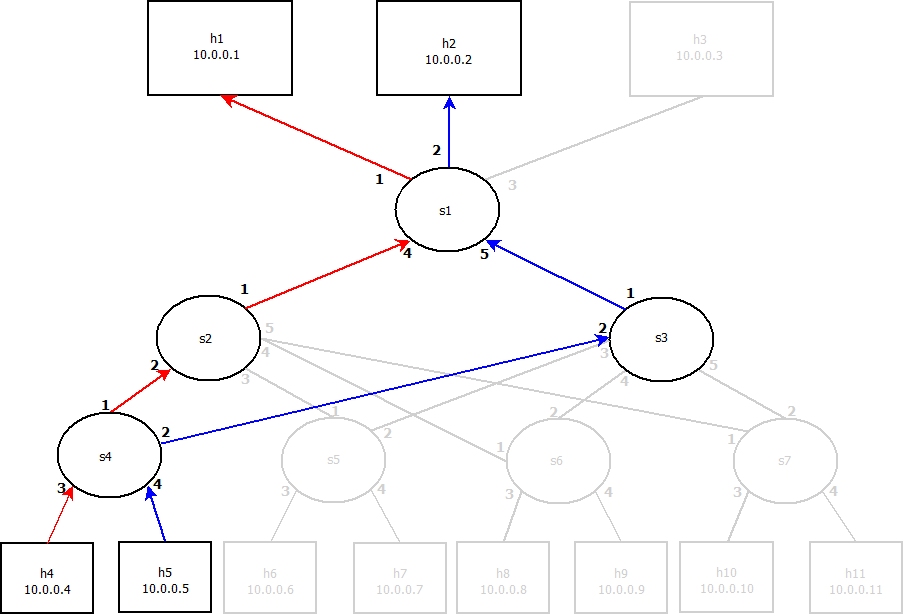
\includegraphics[width=\linewidth]{images/test1.png}
 \caption{Test Case 1: Possible load balanced routes}
 \label{fig:test1}
\end{figure}

\begin{figure}[h]
 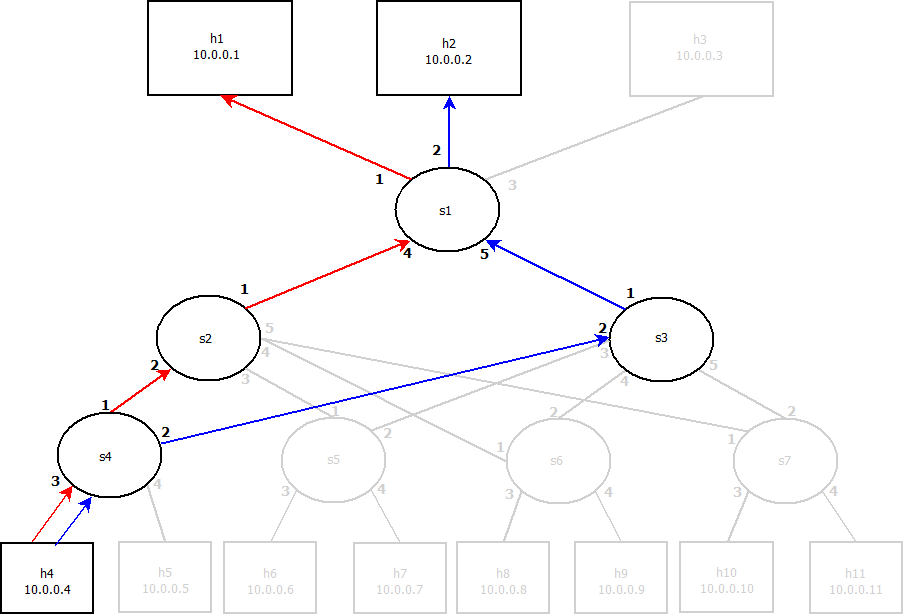
\includegraphics[width=\linewidth]{images/test2.png}
 \caption{Test Case 2: Possible load balanced routes}
 \label{fig:test2}
\end{figure}

\begin{figure}[h]
 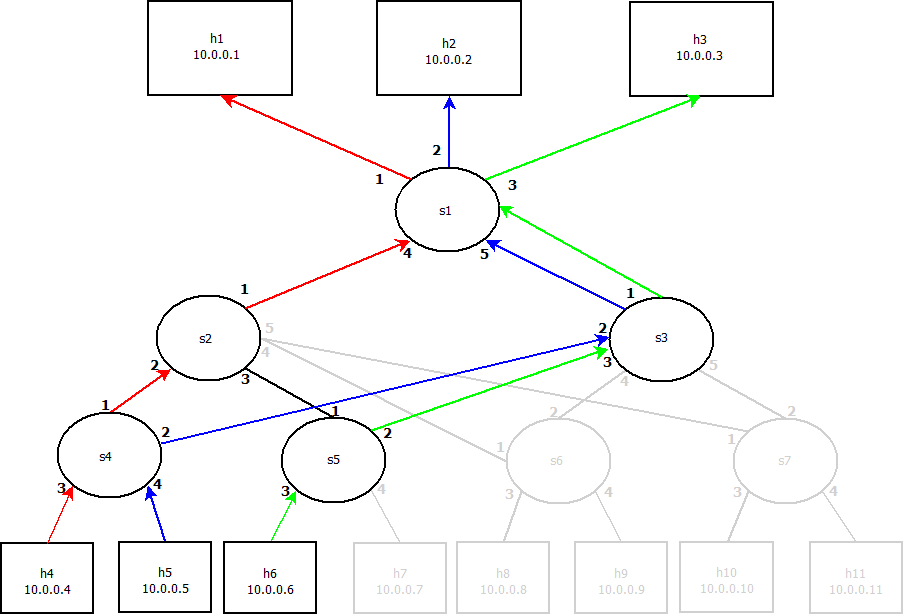
\includegraphics[width=\linewidth]{images/test3.png}
 \caption{Test Case 3: Possible load balanced routes}
 \label{fig:test3}
\end{figure}

\section{Results}
\lipsum[1-1]

\section{Evaluation}
\lipsum[1-1]